\documentclass[11pt,a4paper]{article}
\usepackage[utf8]{inputenc}
\usepackage[ngerman]{babel}
\usepackage{amsmath}
\usepackage{amsfonts}
\usepackage{amssymb}
\usepackage{scrpage2}\pagestyle{scrheadings}
\usepackage[pdftex]{graphicx}
\ihead{Thomas Verweyen (759743) \\ Norman Vetter (749229)}
\setheadsepline{0.2pt}
\begin{document}
\begin{center}
\section*{ Theoretische Informatik 1 \\ Übung Blatt 4}
\end{center}
\ \\ \ \\
\subsection*{Aufgabe 4.1}
\paragraph*{a)}\ \\
$(q_0,baaababaab) \vdash (q_2,aaababaab) \vdash (q_0,aababaab) \vdash (q_1,ababaab) \vdash (q_2,babaab) \vdash (q_1,abaab) \vdash 
(q_2,baab) \vdash (q_1,aab) \vdash (q_2,ab) \vdash (q_0,b) \vdash (q_2,\epsilon)$
\paragraph*{b)}\ \\
$(1)~~(q_0,wv) \vdash^* (q_0,v) \Leftrightarrow (|w|_a - |w|_b)~ mod~ 3 = 0$\\
$(2)~~(q_0,wv) \vdash^* (q_1,v) \Leftrightarrow (|w|_a - |w|_b)~ mod~ 3 = 1$\\
$(3)~~(q_0,wv) \vdash^* (q_2,v) \Leftrightarrow (|w|_a - |w|_b)~ mod~ 3 = 2$\\
\ \\
IA) $w= \epsilon$\\
$(1)~~(q_0,\epsilon v) \vdash^* (q_0,v) \Leftrightarrow (0 - 0) mod 3 = 0$ (ist wahr)\\
$(2)~~\underset{falsch}{\underbrace{(q_0,\epsilon v) \vdash^* (q_1,v)}} \Leftrightarrow \underset{falsch}{\underbrace{(0 - 0)~ mod~ 3 = 0}}$ (Äquivalenz ist wahr)\\
\ \\
$(3)~~\underset{falsch}{\underbrace{(q_0,\epsilon v) \vdash^* (q_2,v)}} \Leftrightarrow \underset{falsch}{\underbrace{(0 - 0)~ mod~ 3 = 0}}$ (Äquivalenz ist wahr)\\
IS:\\
IVor.: (1),(2),(3) gelten für w'.\\
IBeh.: (1),(2),(3) gelten für w mit $w=w'x \wedge x \in \{a,b\}$.\\
IBew.:\\
\ \\
\begin{tabular}{lll}
$(1)(q_0,wv)\vdash^* (q_0,v)$&$ \Leftrightarrow (q_0,w'xv) \vdash^* (q_0,v)$&$ \Leftrightarrow (q_0,w'v) \vdash^* (q_1,v) \wedge x=b$\\
&&\hspace*{3mm}$\vee (q_0,w'v) \vdash^* (q_2,v) \wedge x=a$\\
&&$\Leftrightarrow (|w'|_a-|w'|_b)~mod~3=1 \wedge x=b$\\
&&\hspace*{3mm}$\vee (|w'|_a-|w'|_b)~mod~3=2 \wedge x=a$\\
&&$\Leftrightarrow (|w|_a-|w|_b)~mod~3=0$\\
\end{tabular}
\ \\
\begin{tabular}{lll}
$(2)(q_0,wv) \vdash (q_1,wv)$&$ \Leftrightarrow(q_0,w'xv) \vdash^* (q_1,v)$&$ \Leftrightarrow (q_0,w'v) \vdash^* (q_2,v) \wedge x=b$\\
&&\hspace*{3mm}$\vee (q_0,w'v) \vdash^* (q_0,v) \wedge x=a$\\
&&$\Leftrightarrow (|w'|_a-|w'|_b)~mod~3=2 \wedge x=b$\\
&&\hspace*{3mm}$\vee (|w'|_a-|w'|_b)~mod~3=0 \wedge x=a$\\
&&$\Leftrightarrow (|w|_a-|w|_b)~mod~3=1$
\end{tabular}
\ \\
\begin{tabular}{lll}
$(3)(q_0,wv) \vdash (q_2,wv)$&$ \Leftrightarrow(q_0,w'xv) \vdash^* (q_2,v)$&$ \Leftrightarrow (q_0,w'v) \vdash^* (q_0,v) \wedge x=b$\\
&&\hspace*{3mm}$\vee (q_0,w'v) \vdash^* (q_1,v) \wedge x=a$\\
&&$\Leftrightarrow (|w'|_a-|w'|_b)~mod~3=0 \wedge x=b$\\
&&\hspace*{3mm}$\vee (|w'|_a-|w'|_b)~mod~3=1 \wedge x=a$\\
&&$\Leftrightarrow (|w|_a-|w|_b)~mod~3=2$\\
&&\hfill q.e.d.\\
\end{tabular}
\subsection*{Aufgabe 4.2}
\paragraph*{a)}
$A(L_1)=(\{S,q_0,q_1,q_2,q_3,F\},\{0,1\},\delta,\{F\})$\\
$\delta:$\\
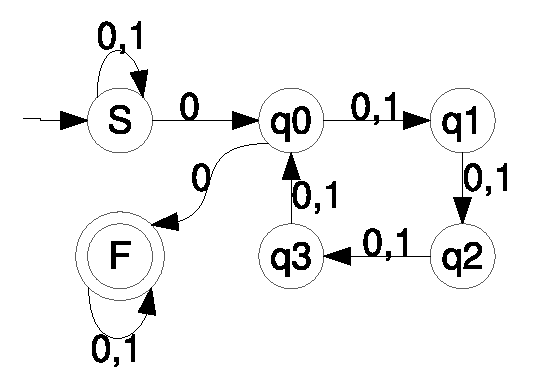
\includegraphics[scale=0.8]{4_2_a.eps}\\
\begin{tabular}{lll}
Zustand&:&Beschreibung\\
S&:&Startzustand mit beliebigem Wort durch Schleifenübergang\\
$q_0$&:&$|u|$ mod 4 = 0\\
$q_1$&:&$|u|$ mod 4 = 1\\
$q_2$&:&$|u|$ mod 4 = 2\\
$q_3$&:&$|u|$ mod 4 = 3\\
F&:&Endzustand\\
\end{tabular}
\paragraph*{b)}
$A(L_2)=(\{S,q_0,q_1,q_2,q_3,q_4,F\},\{a,b,c\},\delta,\{F\})$\\
$\delta:$\\
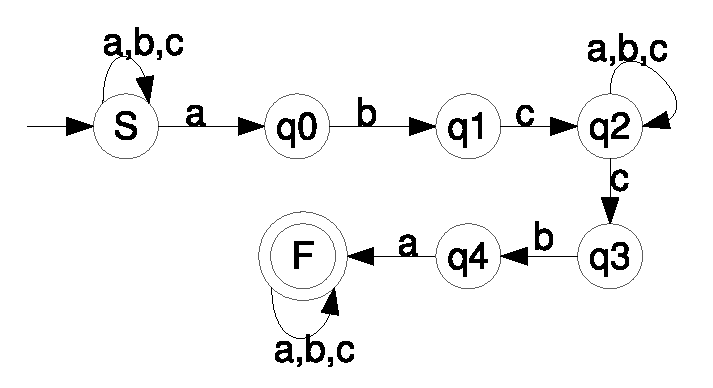
\includegraphics[scale=0.7]{4_2_b.eps}\\
\begin{tabular}{lll}
Zustand&:&Beschreibung\\
S&:&Startzustand mit beliebigem Wort durch Schleifenübergang\\
$q_0$&:&Als Eingabe "'a"' in S bekommen\\
$q_1$&:&Als Eingabe "'b"' in $q_0$ bekommen\\
$q_2$&:&Als Eingabe "'c"' in $q_1$ bekommen,und ist Zustand mit beliebigem Wort\\
&&durch Schleifenübergang\\
$q_3$&:&Als Eingabe "'c"' in $q_2$ bekommen\\
$q_4$&:&Als Eingabe "'b"' in $q_3$ bekommen\\
F&:&Als Eingabe "'a"' in $q_4$ bekommen, und beliebigem Wort\\
&&durch Schleifenübergang, zudem Endzustand\\
\end{tabular}

\subsection*{Aufgabe 4.3}
Gegeben sei der NEA $A=(Q,\Sigma ,\delta, S, F)$.\\
Nun erweitern wir die Menge Q um einen neuen Zustand $q_F$. $Q \cup \{q_F\}$. Dann erweitern wir die Übergangsfunktion $\delta$ um einen $\epsilon$-Übergang für jeden Endzustand zu dem Endzustand $q_F$, und definieren $F=\{q_F\}$.
\end{document}